\section{Results}


We present here the results of the example analysis. Figure \ref{fig:exploratory_analysis} shows the exploratory analysis where the distribution of the response variable is shown on the left and the simulated data are represented on the right.

\begin{figure}
\centering
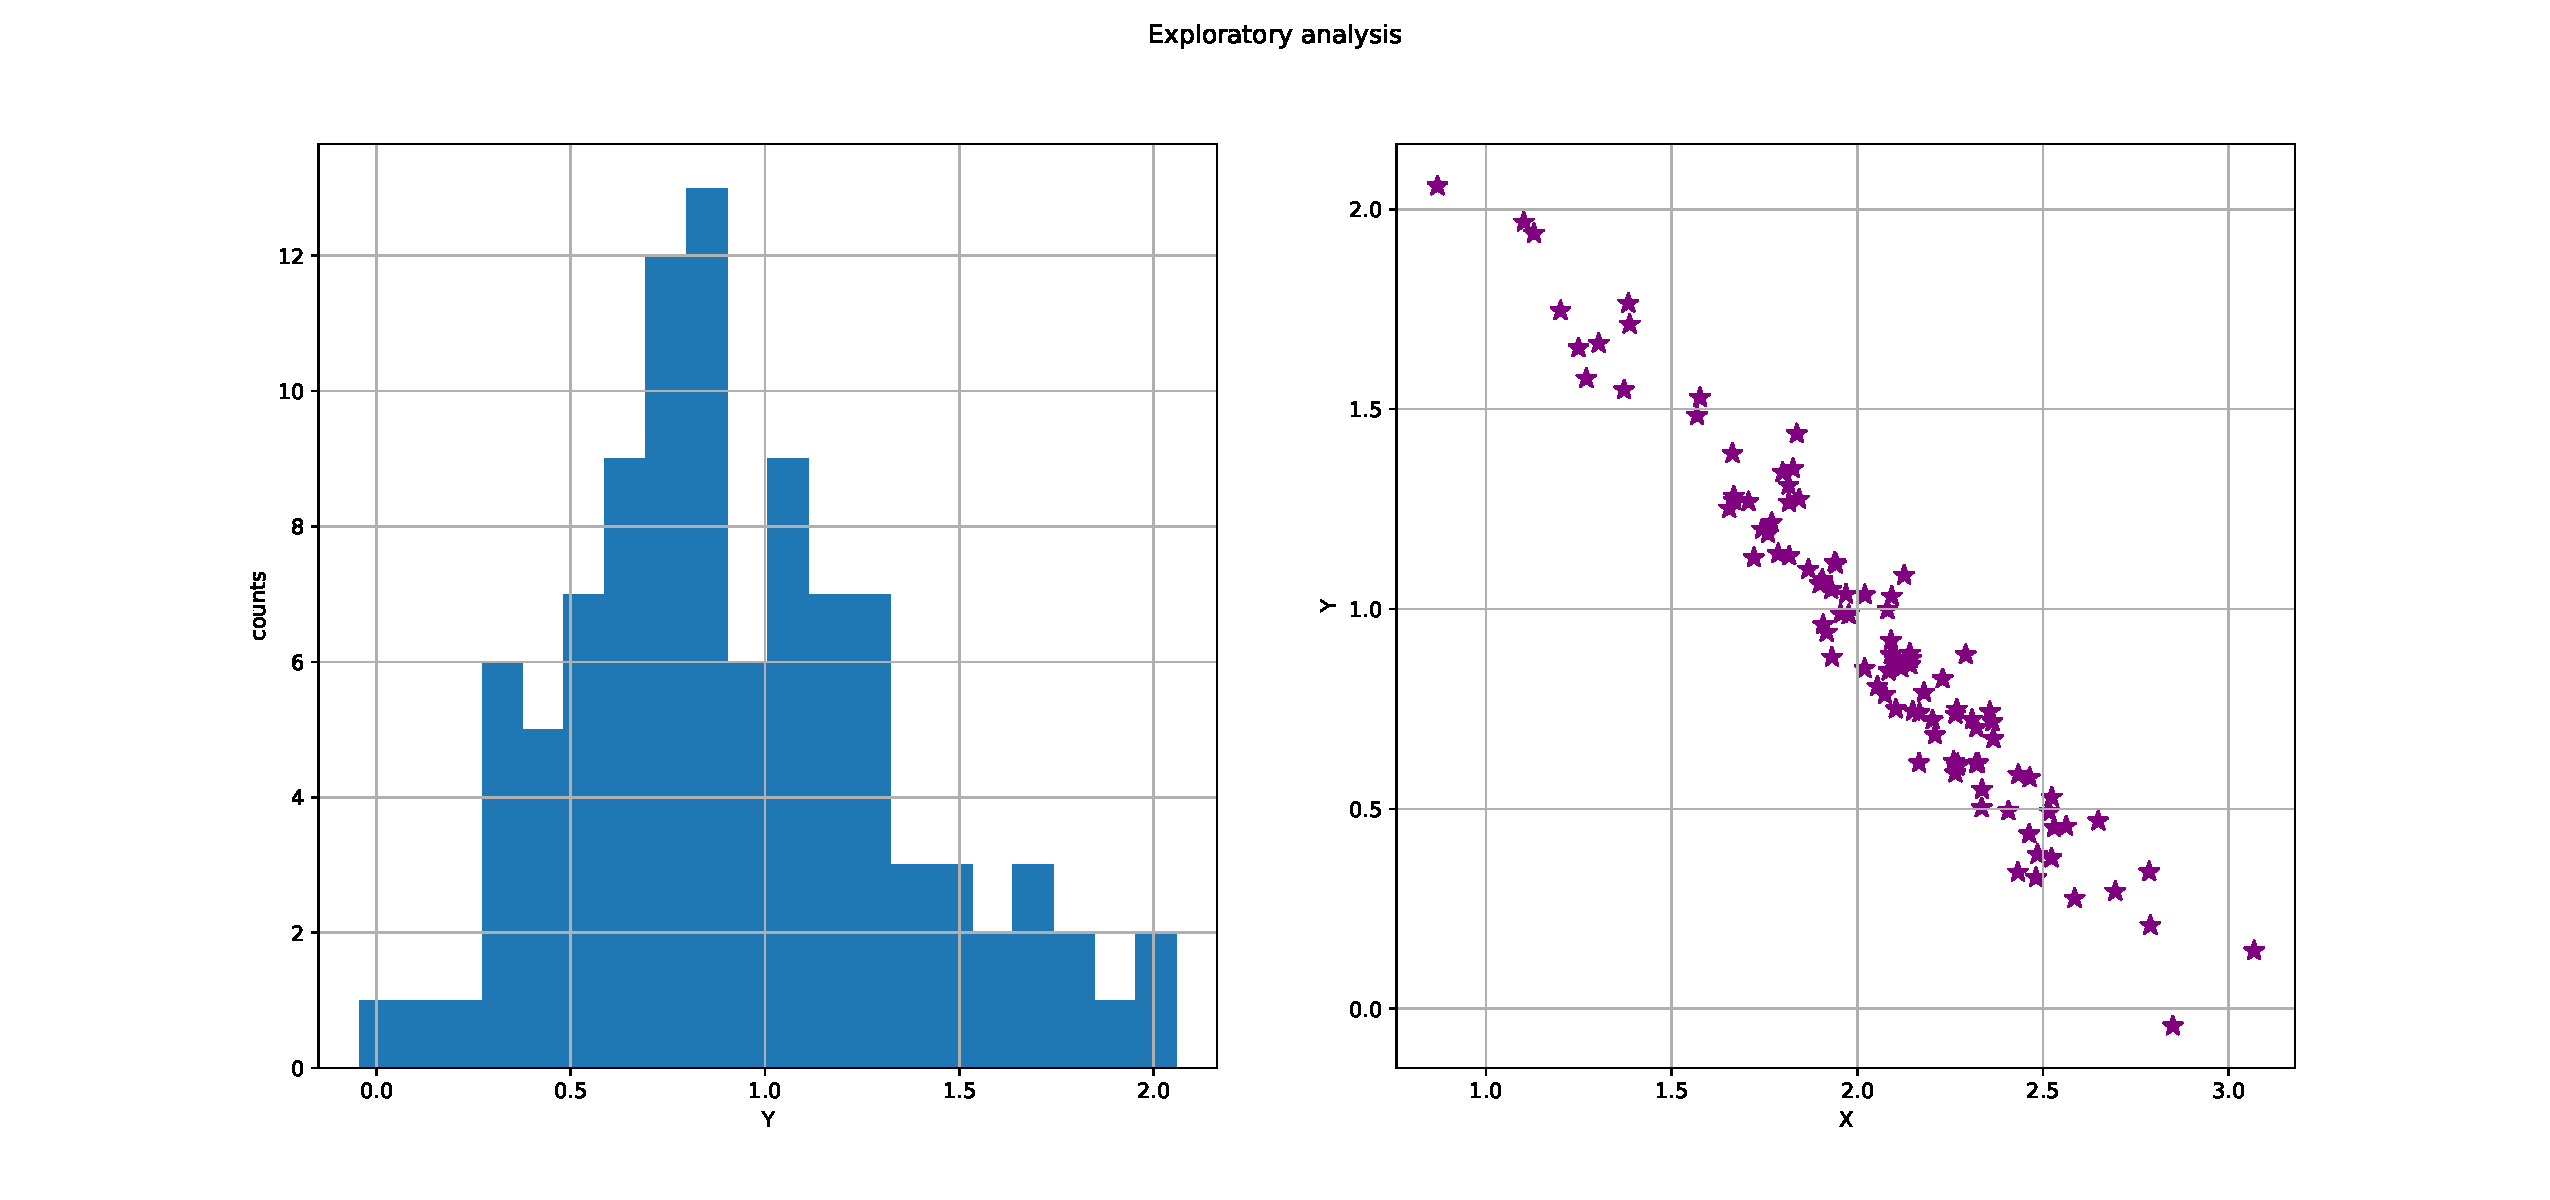
\includegraphics[width=\textwidth]{figures/fig_exploratory_analysis.pdf}
\caption{Exploratory analysis in python}
\label{fig:exploratory_analysis}
\end{figure}

Figure \ref{fig:linear_regression} shows the resulting simple linear regression. The figure on the left shows the fitted regression line where the estimated coefficients fit very well the simulated coefficients on the Python codes. The model presents a good fit as shown on the right figure. That's all.

This is a test to branch "conclusions". TEST BRANCH 1

\begin{figure}
\centering
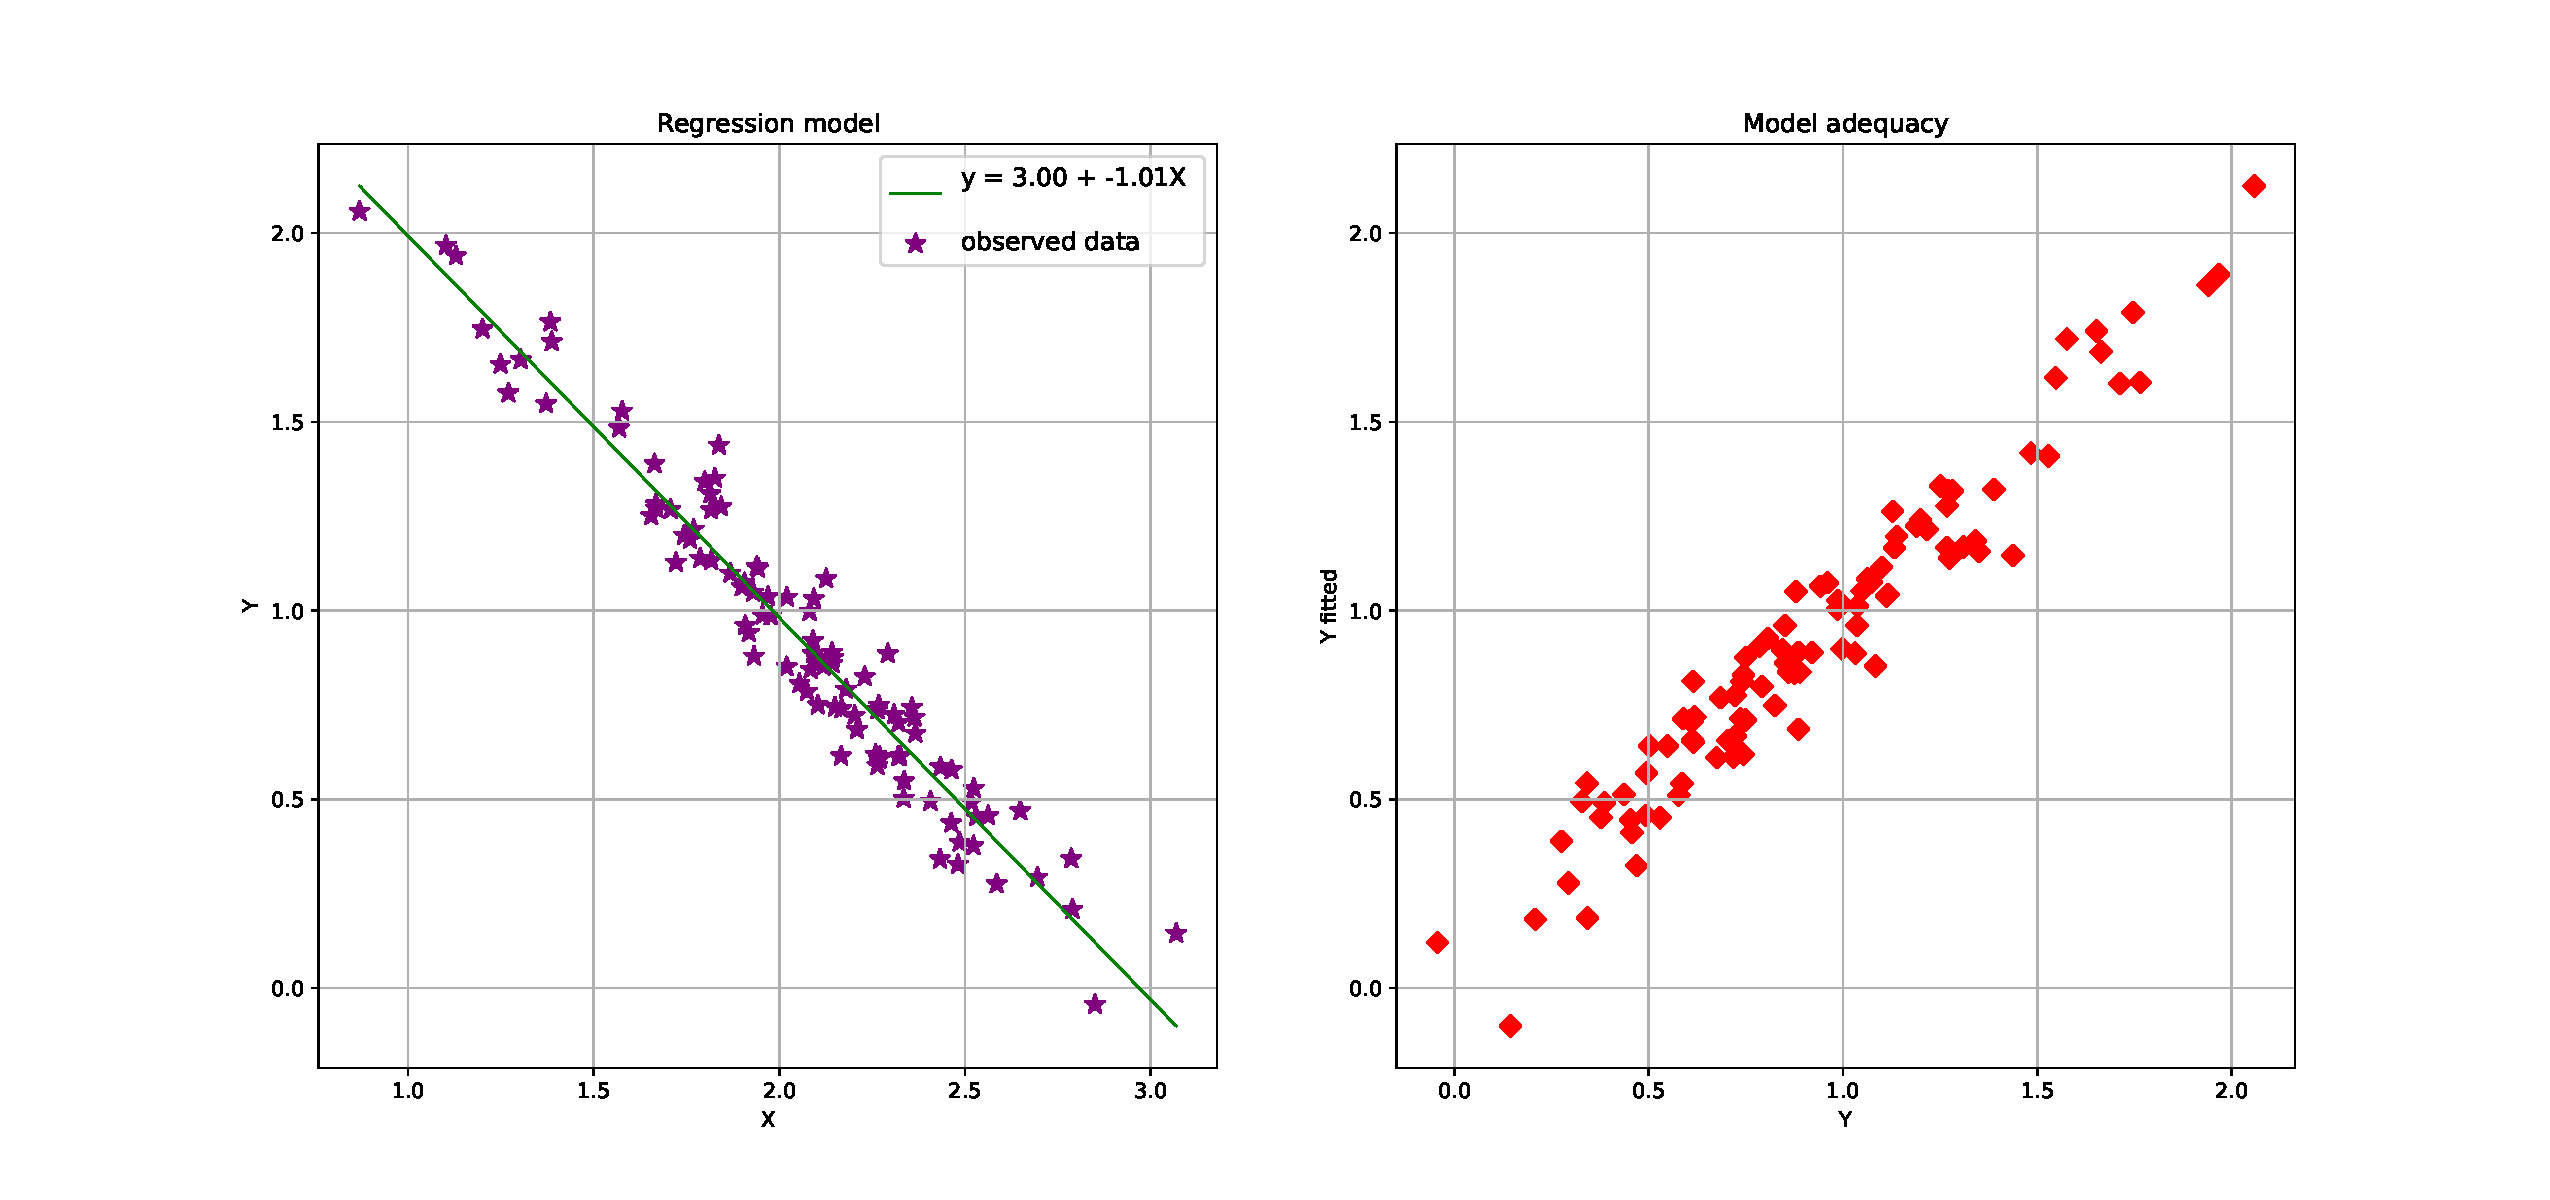
\includegraphics[width=\textwidth]{figures/fig_linear_regression.pdf}
\caption{Linear regression using scikit-learn}
\label{fig:linear_regression}
\end{figure}